\documentclass[10pt,twocolumn,letterpaper]{article}

\usepackage{cvpr}
\usepackage{times}
\usepackage{epsfig}
\usepackage{graphicx}
\usepackage{amsmath}
\usepackage{amssymb}

% Include other packages here, before hyperref.

% If you comment hyperref and then uncomment it, you should delete
% egpaper.aux before re-running latex.  (Or just hit 'q' on the first latex
% run, let it finish, and you should be clear).
\usepackage[breaklinks=true,bookmarks=false]{hyperref}

\cvprfinalcopy % *** Uncomment this line for the final submission

\def\cvprPaperID{****} % *** Enter the CVPR Paper ID here
\def\httilde{\mbox{\tt\raisebox{-.5ex}{\symbol{126}}}}

% Pages are numbered in submission mode, and unnumbered in camera-ready
%\ifcvprfinal\pagestyle{empty}\fi
\setcounter{page}{4321}
\begin{document}

%%%%%%%%% TITLE
\title{CNNs for Single Image Super Resolution}

\author{Michele Bortone\\
{\tt\small michele.bortone@studenti.unipd.it}
% For a paper whose authors are all at the same institution,
% omit the following lines up until the closing ``}''.
% Additional authors and addresses can be added with ``\and'',
% just like the second author.
% To save space, use either the email address or home page, not both
\and
Alessio Lazzaron\\
{\tt\small alessio.lazzaron@studenti.unipd.it}
}

\maketitle
%\thispagestyle{empty}

%%%%%%%%% ABSTRACT
\begin{abstract}
   	Super-resolution is the process of creating high-resolution images from low-resolution images.
   	Single image super-resolution (SISR), refers to the goal of recovering one high-resolution image from one low-resolution image.\\
    In this study we report a comparison between some convolutional neural networks architectures that can solve this task, analyzing its performance. Our goal was to determine if the increase in complexity between the various architectures,  would lead to an increase in performance.\\
    We have analyzed three different architectures and evaluated performance with common image compression quality metrics.
    
\end{abstract}

%%%%%%%%% BODY TEXT
\section{Introduction}

	In most computer vision tasks, high resolution images are usually desired for image processing and analysis. Single Image Super Resolution is widely used in some medical imaging applications (e.g. magnetic resonance imaging), and security and surveillance imaging as well. Moreover, object detection problems can be accomplished using Super-resolution  which helps when low resolution is caused by the long distance between the target and the imaging sensor and objects are too small.
	Super-resolution (SR) refers to the task of restoring high resolution images from one or more low-resolution observations of the same scene. According to the number of input LR images, the SR can be classified into single image super-resolution (SISR) and multi-image super-resolution (MISR). Compared with MISR, SISR is much more popular because of its high efficiency.
	Many SISR methods have been studied in the digital age, including interpolation tecniques such as Nearest neighbor or bicubic.\\
	Recent popular methods are based on neural networks and most architectures studied for thi task are Convolutional Neural networks and Deep Generative models.\\
	The deep learning models capability is particularly suitable for this type of task because simpler approaches like bicubic interpolation use only local information in an LR image to compute pixel values in the corresponding SR image, deep learning approaches, on the other hand, learn mapping functions from LR images to HR images from a large number of examples.\\
	
\section{Related work}
	Deep learning can be used to estimate the High Resolution (HR) image given a Low Resolution (LR) image. By using the HR image as a target (or ground-truth) and the LR image as an input, we can treat this like a supervised learning problem. There are a lot of approaches to affront this problem however most of them use CNNs because they get better performances.  Some approaches are listed below and represent a broad outline of the current state of the art.
\subsection{Pre-upsampling}
	In this method, the low-resolution images are first interpolated to obtain a “coarse” high resolution image. Now, CNNs are used to learn an end-to-end mapping from the interpolated low resolution images to the high resolution images. The intuition was that it may be easier to first upsample the low-resolution images using traditional methods (such as Bicubic interpolation) and then refine the resultant than learn a direct mapping from a low-dimensional space to a high-dimensional space. The advantage is that since the upsampling is done by traditional methods, the CNN only needs to learn how to refine the coarse image, which is simpler.\\
	In our comparison, we implemented and analyzed two pre-upsampling networks, that are SRCNN \cite{dong2014image} (Super Resolution Convolutional Neural Network) and VDSR \cite{kim2015accurate} (Very Deep Super Resolution).
\subsection{Post-upsampling}
	This method works in reverse way respect to the previous one, indeed the low-resolution images are passed to the CNNs as such. Upsampling is performed in the last layer using a learnable layer. The advantage of this method is that feature extraction is performed in the lower dimensional space (before upsampling) and hence the computational complexity is reduced. Also, by using an learnable upsampling layer, the model can be trained end-to-end.\\
	This network architecrture is suitable when we are interested to produce the output quickly because we can skip the pre-upsampling process.
	In this this report we have compared FSRCNN \cite{dong2016accelerating} (Fast Super Resolution Convolutional Neural Network) with the two Pre-upsampling CNNs cited above.
\subsection{Progressive upsampling}
The above approaches use only a single upsampling convolution to not increase the computational complexity. This makes the learning process harder for large scaling factors. To avoid it these models  use a cascade of CNNs to progressively reconstruct high resolution images. By decomposing a difficult task into simpler tasks, the learning difficulty is greatly reduced and better performance can be obtained.
\subsection{Iterative Up and Down sampling}
Another popular model architecture is the hourglass structure that alternating between the process of upsampling and downsampling. These models can better find the deep relations between the LR-HR image pairs and thus provide higher quality reconstruction results.
\subsection{Generative Adversarial Networks (GANs)}
This type of network have been increasingly used for several image based applications including Super Resolution. GANs typically is composed of two neural networks: the Generator and the Discriminator, that dueling each other in a zero-sum game. Given a set of target samples, the Generator tries to produce samples that can fool the Discriminator into believing they are real. The Discriminator tries to recognize the real (target) samples from fake (generated) samples. At the end we obtain a Generator that is really good at generating samples similar to the target samples.

\section{Dataset}
For our purpose we use three different dataset for the training phase, the first is \textit{T91} that is the smallest dataset, it contains 91 mixed images of small size that representing fruits, vegetables, objects and people. The second is \textit{General100} that contains 100 bmp-format images with no compression. The size of these 100 images ranges from 710 x 704, the largest, to 131 x 112, the smallest. And the third dataset is \textit{Berkeley Segmentation Dataset (BSDS200)}, ot contain 200 images and it is created for developing new boundary detection algorithms and for developing a benchmark for that task. For each neural network that we implement, we also adjust the number of epochs for the training phase, in fact, since the size of the datasets were different it was necessary to customize this hyperparameters to have, more or less, the same performances on the validation test and avoid overfitting. The validation set is obtained by split the dataset in two parts: the biggest one, almost the 80\% of the dataset, for the training set, and the rest 20\% for the validation set. However using different type of training set didn't change the models performance so much.\\
To testing the performance of the models and to understand how much the models are able to reconstruct from the low-resolution images to high resolution images we use, as testing dataset, \textit{Set5} and \textit{Set14} that are common evaluation dataset  for Super Resolution task and contains various images of buildings to animal faces.\\
Official web pages of SRCNN, FSRCNN and VDSR provide all datasets used.
We don’t use directly the dataset but we apply some preprocessing. First off all we convert the training set’s images from RGB into YCbCr format because the models is training with only the luma, the brightness, of the images. After this, we normalize the images in order to have floating point values between 0 and 1, so in this way we make the convergence of the loss function faster. The low-resolution images is made by down and up sampling the images, inside the dataset, with a bicubic interpolation and we analyze the model’s performance with different scale factors.\\
In order to perform training operations with larger dataset we do some data augmentation. 
We crop small images called patches from each image in the training set. Patches are overlapping sub-images densely cropped from the original image with low size. The stride which controls how many images are cropped and size are hyperparameters.\\
Patch extraction is the process of extracting a large set of small image patches,  from a single larger image. This type of data augmentation is frequently used in image-to-image regression problems such as Super Resolution, where networks can be trained on very small input image sizes.
Patch extraction is widely used  in recent Super Resolution methods.\\
Also in deep models we use rotated images to create a larger dataset for the training phase.\\


\section{Method}
We want to verify if the complexity of the model increases also its performance do too. So we implement three convolutional neural network that are different for the complexity of the architecture.
\subsection{SRCNN}
The Super Resolution CNN is a convolutional neural network with three layer where the first layer has 64 filters and each of them as a dimension of 9x9, the second layer has 32 filters with dimension 1x1 and the output layer has only one filter with dimension 5x5. Every layer not have padding and for the first two layer we use a relu activation function and for the last layer we adopt a linear activation function. The loss, that the model want to minimize is the mean square error between the low resolution images and the output high resolution images, and it does this using stochastic gradient descent with the standard backpropagation. More precisely we adopt Adam as optimization algorithm 
\begin{figure}[htp]
    \centering
    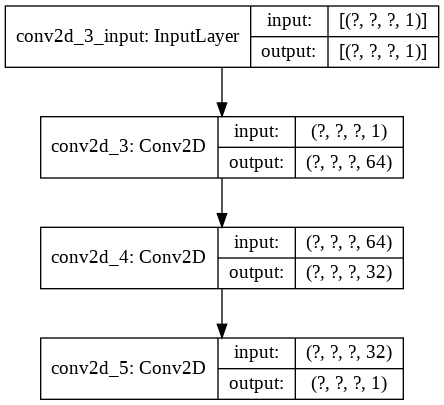
\includegraphics[scale=0.4]{img/srcnn.png}
    \label{fsrcnn}
    \caption{Archittettura SRCNN}
\end{figure}
\subsection{FSRCNN}
FSRCNN is presented by the authors like an evolution of SRCNN. The main goal of this architecture is to reduce the the time complexity of the output image computation.\\
To solve the computational cost problem, the bicubic interpolation step computed in SRCNN is replaced with a deconvolutional layer. In FSRCNN there is no pre-processing and the the input is the low resolution image.\\
As shown in figure \ref{fsrcnn}, FSRCNN is composed by five main parts:
\begin{itemize}
	\item \textbf{Feature Extraction:} performs feature extraction on ththe low resolution image;
	\item \textbf{Shrinking:} reduces the number of feature maps so parameters as well;
	 \item \textbf{Non-Linear Mapping:} multiple layers that map feature maps to high resolution  representation;
	\item \textbf{Expanding:} Inverse process of the shrinking layer;
	\item \textbf{Deconvolution;} aggregates features and create upsampled image.
\end{itemize}
We can see the deconvolution operation like the inverse of the convolution. The output of this layer will be the input size multiplied by the stride.  The stride of the deconvolutional operation is set to the desired upscaling factor.\\
Another way to see the deconvolution operation is to think it like an upsampling method such as interpolation but with parameters to learn with optimization algorithms.\\
The number of filters on feature extraction \textit{d}, the number of filters after shrinking operation \textit{s} and the number of non-linear mapping layers \textit{m} are hyperparameters.\\
The non-linear mapping step in SRCNN is replaced by shrinking, mapping, and expanding step.
The non-linear mapping operation is composed by multiple smaller layers than the single wide layer used in SRCNN, so this operation is more efficient due to the deep networks advantages.\\
Finally shrinking and expanding operations are able to reduce drastically the number of parameters to learn during training. Smaller number of parameters and the low resolution input produce a faster output than SRCNN.\\


\begin{figure*}[!]
	\centering
	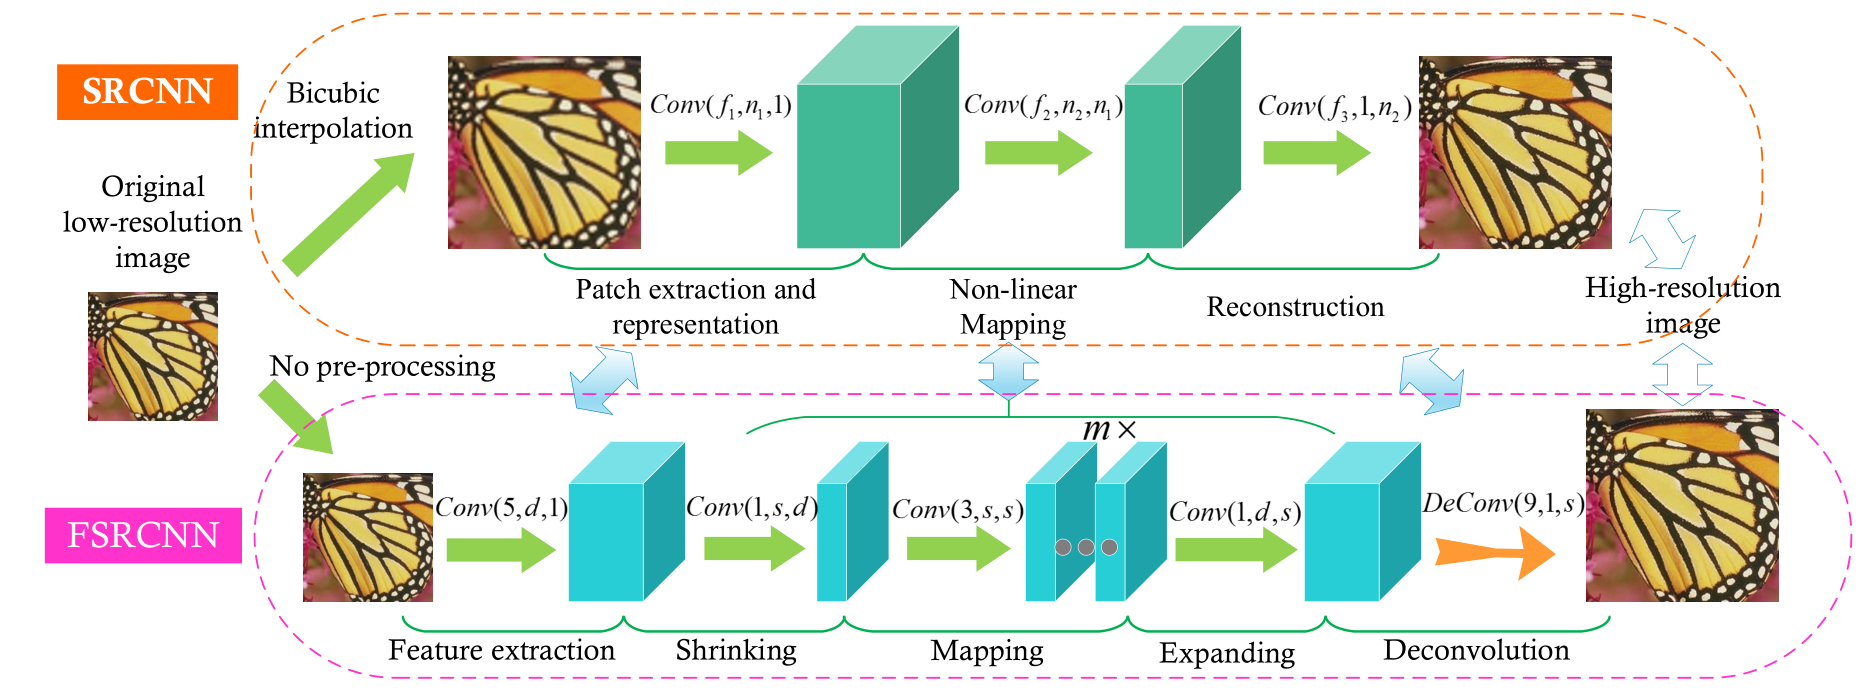
\includegraphics[width=\textwidth]{img/fsrcnn.png}
	\caption{Comparison between SRCNN and FSRCNN architectures \cite{dong2014image}}
\end{figure*}

\subsection{VDSR}



\section{Experiments}

\section{Conclusion}


\subsection{Suggested Structure}

The following is a suggested structure for your report:

\begin{itemize}
	\item Introduction (10\%): describe the problem you are working on, why it's important, and an overview of your results.
	\item Related Work (10\%): discuss published work or similar apps that relates to your project. How is your approach similar or different from others?
	\item Dataset (15\%): describe the data you are working with for your project. What type of data is it? Where did it come from? How much data are you working with? Did you have to do any preprocessing, filtering, etc., and why?
	\item Method (30\%): discuss your approach for solving the problems that you set up in the introduction. Why is your approach the right thing to do? Did you consider alternative approaches? It may be helpful to include figures, diagrams, or tables to describe your method or compare it with others.
	\item Experiments (30\%): discuss the experiments that you performed. The exact experiments will vary depending on the project, but you might compare with prior work, perform an ablation study to determine the impact of various components of your system, experiment with different hyperparameters or architectural choices. You should include graphs, tables, or other figures to illustrate your experimental results.
	\item Conclusion (5\%): summarize your key results; what have you learned? Suggest ideas for future extensions.
\end{itemize}	

%------------------------------------------------------------------------
\section{Formatting your paper}

All text must be in a two-column format. The total allowable width of the
text area is $6\frac78$ inches (17.5 cm) wide by $8\frac78$ inches (22.54
cm) high. Columns are to be $3\frac14$ inches (8.25 cm) wide, with a
$\frac{5}{16}$ inch (0.8 cm) space between them. The main title (on the
first page) should begin 1.0 inch (2.54 cm) from the top edge of the
page. The second and following pages should begin 1.0 inch (2.54 cm) from
the top edge. On all pages, the bottom margin should be 1-1/8 inches (2.86
cm) from the bottom edge of the page for $8.5 \times 11$-inch paper; for A4
paper, approximately 1-5/8 inches (4.13 cm) from the bottom edge of the
page.

%-------------------------------------------------------------------------
\subsection{Margins and page numbering}

All printed material, including text, illustrations, and charts, must be kept
within a print area 6-7/8 inches (17.5 cm) wide by 8-7/8 inches (22.54 cm)
high.
Page numbers should be in footer with page numbers, centered and .75
inches from the bottom of the page and make it start at the correct page
number rather than the 4321 in the example.  To do this fine the line (around
line 23)
\begin{verbatim}
%\ifcvprfinal\pagestyle{empty}\fi
\setcounter{page}{4321}
\end{verbatim}
where the number 4321 is your assigned starting page.

Make sure the first page is numbered by commenting out the first page being
empty on line 46
\begin{verbatim}
%\thispagestyle{empty}
\end{verbatim}


%-------------------------------------------------------------------------
\subsection{Type-style and fonts}

Wherever Times is specified, Times Roman may also be used. If neither is
available on your word processor, please use the font closest in
appearance to Times to which you have access.

MAIN TITLE. Center the title 1-3/8 inches (3.49 cm) from the top edge of
the first page. The title should be in Times 14-point, boldface type.
Capitalize the first letter of nouns, pronouns, verbs, adjectives, and
adverbs; do not capitalize articles, coordinate conjunctions, or
prepositions (unless the title begins with such a word). Leave two blank
lines after the title.

AUTHOR NAME(s) and AFFILIATION(s) are to be centered beneath the title
and printed in Times 12-point, non-boldface type. This information is to
be followed by two blank lines.

The ABSTRACT and MAIN TEXT are to be in a two-column format.

MAIN TEXT. Type main text in 10-point Times, single-spaced. Do NOT use
double-spacing. All paragraphs should be indented 1 pica (approx. 1/6
inch or 0.422 cm). Make sure your text is fully justified---that is,
flush left and flush right. Please do not place any additional blank
lines between paragraphs.

Figure and table captions should be 9-point Roman type as in
Table~\ref{mytable}. Short captions should be centred.

\noindent Callouts should be 9-point Helvetica, non-boldface type.
Initially capitalize only the first word of section titles and first-,
second-, and third-order headings.

FIRST-ORDER HEADINGS. (For example, {\large \bf 1. Introduction})
should be Times 12-point boldface, initially capitalized, flush left,
with one blank line before, and one blank line after.

SECOND-ORDER HEADINGS. (For example, { \bf 1.1. Database elements})
should be Times 11-point boldface, initially capitalized, flush left,
with one blank line before, and one after. If you require a third-order
heading (we discourage it), use 10-point Times, boldface, initially
capitalized, flush left, preceded by one blank line, followed by a period
and your text on the same line.

%-------------------------------------------------------------------------
\subsection{Footnotes}

Please use footnotes\footnote {This is what a footnote looks like.  It
often distracts the reader from the main flow of the argument.} sparingly.
Indeed, try to avoid footnotes altogether and include necessary peripheral
observations in
the text (within parentheses, if you prefer, as in this sentence).  If you
wish to use a footnote, place it at the bottom of the column on the page on
which it is referenced. Use Times 8-point type, single-spaced.


%-------------------------------------------------------------------------
\subsection{References}

List and number all bibliographical references in 9-point Times,
single-spaced, at the end of your paper. When referenced in the text,
enclose the citation number in square brackets, for
example~\cite{Authors14}.  Where appropriate, include the name(s) of
editors of referenced books.

\begin{table}
\begin{center}
\begin{tabular}{|l|c|}
\hline
Method & Frobnability \\
\hline\hline
Theirs & Frumpy \\
Yours & Frobbly \\
Ours & Makes one's heart Frob\\
\hline
\end{tabular}
\end{center}
\caption{Results. Ours is better.}
\label{mytable}
\end{table}

%-------------------------------------------------------------------------
\subsection{Illustrations, graphs, and photographs}

All graphics should be centered.  Please ensure that any point you wish to
make is resolvable in a printed copy of the paper.  Resize fonts in figures
to match the font in the body text, and choose line widths which render
effectively in print.  Many readers (and reviewers), even of an electronic
copy, will choose to print your paper in order to read it.  You cannot
insist that they do otherwise, and therefore must not assume that they can
zoom in to see tiny details on a graphic.

When placing figures in \LaTeX, it's almost always best to use
\verb+\includegraphics+, and to specify the  figure width as a multiple of
the line width as in the example below
{\small\begin{verbatim}
   \usepackage[dvips]{graphicx} ...
   \includegraphics[width=0.8\linewidth]
                   {myfile.eps}
\end{verbatim}
}


{\small
\bibliographystyle{ieee_fullname}
\bibliography{project_report_bib}
}

\end{document}
